\documentclass[10pt]{article}
\usepackage{icmlko}

\icmlmeta{IP 파운데이션 월드모델}{160}{축의 방향을 라벨로 정하고 있었다}{입장 마찰만 어느 통제로도 안 고쳐지는 이유를 쫓다가, 그 축이 여섯 도메인에서 라벨에 맞춰 미리 뒤집혀 있는 것을 찾았다 --- 그중 하나가 유보 라벨을 봐야만 정할 수 있는 결정이었다}

\begin{document}

\twocolumn[
\icmlheader

\begin{abstract}
노트 159가 ``입장 마찰만 어느 통제로도 안 고쳐진다(능형 0/8)''를 남겼다.
쫓아갔다. \textbf{먼저 내 검정이 순환이었다.} 하네스의
\texttt{entry\_friction} 열은 원자료와 상관이 $-$1.0이다 --- 노트 108이 채택한
\texttt{axis\_orient.json} 이 여섯 도메인(도서 · 모바일 · 애니 · 웹툰 · 팝업 ·
펀딩)에서 축을 뒤집고 있었고, \textbf{뒤집을지는 라벨과의 상관 부호로
정했다.} 라벨에 맞춰 정렬된 열에 ``입장 마찰은 내려가야 한다''는 사전 부호를
대면 당연히 0/8이 나온다. 재는 대상이 아니라 규약을 재고 있었다.
\textbf{그런데 규약 자체에 구멍이 있었다.} 방향을 각 도메인의 \emph{학습
기간만}으로 다시 정해 보니 아홉 중 넷이 어긋난다. 만화 · 세계애니는 상관이
$-$0.034로 문턱 아래라 안 뒤집은 것이고, 애니는 학습 기간에서 $+$0.037이라
안 뒤집어야 하는데 뒤집혀 있다(전체로는 $-$0.086). \textbf{그리고 팝업은
2025년 이전 관측이 16건이라 상관이 아예 정의되지 않는다} --- 즉 팝업의
뒤집기는 \textbf{유보 기간 라벨을 봐야만 나오는 결정}이었다. 값을 쟀다.
팝업의 뒤집기를 되돌리면 팝업 $\rho$ 가 F18 배깅에서 $+$0.4517에서
\textbf{$+$0.3388}로, 능형에서 $+$0.5167에서 \textbf{$+$0.4286}으로 내려간다
--- \textbf{헤드라인이 0.113 · 0.088 만큼 부풀어 있었다.} 판 $\rho$ 는
$-$0.003 밖에 안 움직여 순위표는 그대로다. 되돌렸고, 규약을 적었다:
\textbf{축 방향을 라벨로 정할 때는 학습 기간만 본다. 학습 기간으로 못 정하는
도메인은 뒤집지 않는다}(노트 141의 ``모르면 막는다''). 그리고 원자료로
다시 보면 입장 마찰의 원래 관계는 여덟 도메인 중 일곱에서 음수이고 팝업도
$-$0.246이다 --- \textbf{내 사전 부호가 맞았고, 자료가 그것을 뒤집어 놓았던
것이다.}
\end{abstract}
]

\begin{figure*}[t]
\centering
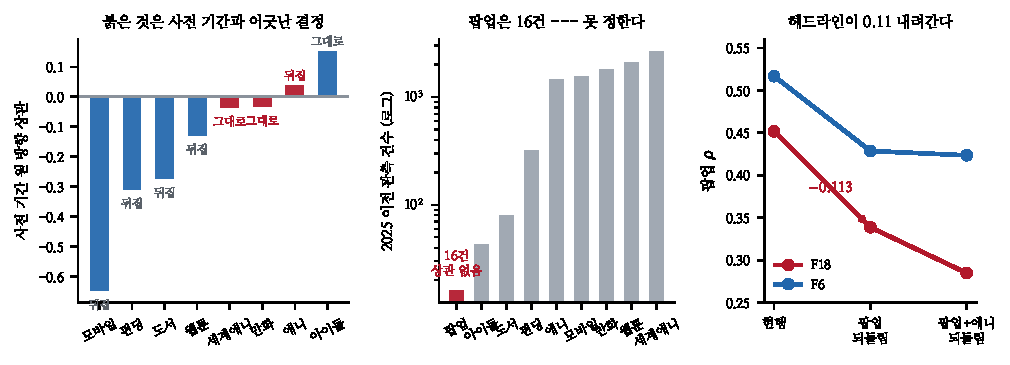
\includegraphics[width=\textwidth]{figs/orient.pdf}
\caption{왼쪽 --- 붉은 것은 학습 기간과 어긋난 결정. 가운데 --- 팝업은
16건이라 못 정한다. 오른쪽 --- 되돌리면 헤드라인이 0.11 내려간다.}
\end{figure*}

\section{내 검정이 순환이었다}

\claimx{\textbf{하네스의 \texttt{entry\_friction} 은 원자료의 반대다.}
\texttt{state/tri\_domain.py} 의 \texttt{\_apply\_adopted} 가
\texttt{axis\_orient.json} 을 읽어 여섯 도메인에서 값 $\to$ $1-$값을 한다.
노트 155부터 159까지 ``입장 마찰이 사전 부호와 안 맞는다''를 다섯 노트에
걸쳐 적었는데, \textbf{뒤집힌 열에 안 뒤집힌 사전 부호를 댄 것}이다.}{다섯
축 중 이 축만 그렇다 --- 나머지 넷은 원자료와 그대로 일치한다.
\texttt{media\_push} 도 애니 하나만 뒤집혀 있다.}

\section{규약에 구멍이 있었다}

\begin{table}[t]
\centering\tsize
\caption{방향을 학습 기간(2025 이전)만으로 다시 정하면.}
\begin{tabular}{lrrrl}
\toprule
& 현행 & 사전 n & 사전 상관 & 사전 결정 \\
\midrule
모바일 & 뒤집 & 1{,}559 & $-$.648 & 뒤집 \\
펀딩 & 뒤집 & 320 & $-$.310 & 뒤집 \\
도서 & 뒤집 & 80 & $-$.273 & 뒤집 \\
웹툰 & 뒤집 & 2{,}106 & $-$.129 & 뒤집 \\
아이돌 & 그대로 & 43 & $+$.152 & 그대로 \\
\midrule
\textbf{애니} & \textbf{뒤집} & 1{,}467 & \textbf{$+$.037} & \textbf{그대로} \\
만화 & 그대로 & 1{,}783 & $-$.034 & 뒤집 \\
세계애니 & 그대로 & 2{,}648 & $-$.036 & 뒤집 \\
\textbf{팝업} & \textbf{뒤집} & \textbf{16} & \textbf{없음} & \textbf{그대로} \\
\bottomrule
\end{tabular}
\end{table}

\claimx{\textbf{팝업은 자기 학습 기간으로 방향을 정할 수가 없다.} 2025년
이전 관측이 16건이고 상관이 정의되지 않는다. 그런데 뒤집혀 있다 ---
\textbf{유보 기간 라벨을 봐야만 나오는 결정}이다.}{만화 · 세계애니가
안 뒤집힌 것은 상관이 $-$0.034로 작아 노트 108의 문턱을 못 넘은 것이고,
애니는 전체로는 $-$0.086이라 넘었지만 학습 기간만 보면 $+$0.037이다.
\textbf{넷 중 셋은 문턱 문제이고 팝업 하나만 원리적으로 못 정한다.}}

\section{값을 쟀다}

\begin{table}[t]
\centering\tsize
\caption{팝업의 뒤집기를 되돌리면.}
\begin{tabular}{lrrrr}
\toprule
& \multicolumn{2}{c}{F18 배깅} & \multicolumn{2}{c}{F6 능형} \\
& 판 & \textbf{팝업} & 판 & \textbf{팝업} \\
\midrule
현행 & $+$.4491 & \textbf{$+$.4517} & $+$.3671 & \textbf{$+$.5167} \\
\textbf{팝업 되돌림} & $+$.4465 & \textbf{$+$.3388} & $+$.3651 & \textbf{$+$.4286} \\
팝업$+$애니 되돌림 & $+$.4488 & $+$.2849 & $+$.3592 & $+$.4235 \\
\bottomrule
\end{tabular}
\end{table}

\claimx{\textbf{헤드라인이 0.113 부풀어 있었다.} 팝업 $\rho$ 가 F18 에서
$+$0.4517 $\to$ $+$0.3388, 능형에서 $+$0.5167 $\to$ $+$0.4286이다. 판
$\rho$ 는 $-$0.003 밖에 안 움직여 순위표와 챔피언은 그대로다.}{크기가 유보
59건의 짝 반폭(0.12)과 비슷해 ``통계적으로 갈린다''고까지는 못 한다. 다만
이건 크기 문제가 아니라 \textbf{규약 문제}다 --- 유보 라벨로 자질의 부호를
정하면 안 된다.}

\claimx{\textbf{애니까지 되돌리면 팝업이 더 내려간다}($+$0.339 $\to$
$+$0.285). 팝업의 축이 아닌데 팝업이 움직이는 것은 풀링 전파다(노트 144의
귀착).}{그래서 애니는 따로 재야 한다 --- 사전 $n{=}1{,}467$ 이라 팝업과는
다른 사안이고, 문턱을 어디 두느냐의 문제다.}

\section{그리고 내 사전 부호가 맞았다}

\begin{table}[t]
\centering\tsize
\caption{원 방향(뒤집기 전) 입장 마찰과 라벨의 상관.}
\begin{tabular}{lrl}
\toprule
모바일 & $-$.578 & \\
도서 & $-$.297 & \\
\textbf{팝업} & \textbf{$-$.246} & 유보 59건 \\
펀딩 & $-$.256 & \\
애니 & $-$.086 & \\
만화 · 세계애니 & $-$.034 & \\
웹툰 & $-$.019 & \\
\bottomrule
\end{tabular}
\end{table}

\claimx{\textbf{입장 마찰은 원래 여덟 중 일곱에서 음수다.} 유료 · 사전예약
장벽이 높을수록 일평균 방문객이 적다 --- 사전 부호 $-1$ 이 맞았다. 노트
155에서 ``내 상식이 틀렸나''를 의심했는데, 틀린 것은 상식이 아니라 자료
쪽 규약이었다.}{그렇다고 이것이 인과라는 뜻은 아니다. 노트 155의 선택 설명
(``유료를 거는 팝업은 원래 수요가 있다'')은 여전히 가능하고, 그 방향이면
관측 상관이 더 음수여야 한다.}

\section{고치고 적었다}

\texttt{axis\_orient.json} 에서 팝업을 뺐고
\texttt{data/state/axis\_orient\_note.md} 에 무엇을 왜 정했는지 적었다.

\claimx{\textbf{규약: 축 방향을 라벨로 정할 때는 학습 기간만 본다. 학습
기간으로 못 정하는 도메인은 뒤집지 않는다.}}{노트 141의 ``모르면 막는다''
와 같은 형태다. 그때는 시점을 몰라서 막았고 이번엔 방향을 몰라서 안 뒤집는다.}

\begin{table}[t]
\centering\tsize
\caption{남은 것.}
\begin{tabular}{ll}
\toprule
애니 & 문턱을 어디 두나 --- 사전 $+$.037 대 전체 $-$.086 \\
다른 축 & 방향을 라벨로 정한 곳이 또 있나 (media\_push 애니) \\
\textbf{다섯 노트} & 155$\sim$159의 입장 마찰 서술을 다시 읽을 것 \\
\bottomrule
\end{tabular}
\end{table}

마지막 줄이 부채다. 노트 155부터 159까지 입장 마찰을 ``어느 통제로도 안
고쳐지는 축''으로 다섯 번 적었다. 그 서술은 전부 뒤집힌 열을 본 것이다.
\textbf{방향을 바로잡고 다시 재면 입장 마찰이 제일 잘 맞는 축일 수도 있다}
--- 그것이 다음 실험이다.

\end{document}
